\chapter{BACKGROUND AND RELATED WORK}
\label{chap:bgrw}
In this chapter, we describe in detail the generational GP algorithm(\citep{poli08:fieldguide},\citep{RFIgp2016}), which serves as a base for our parallelization experiments in \Cref*{chap:ourwork}. Later on, we also give a brief description of existing work which also parallelizes this algorithm.

Note that throughout this chapter, the terms program and expression tree are interchangable, since we are using GP for symbolic regression. 

\section{The Generational GP Algorithm}
\label{bgrw:algo}
The generational GP algorithm gives us a method to evolve candidate programs using the principles of natural selection. There are $3$ main steps involved in the algorithm. 
\begin{itemize}
  \item Selection - In this step, we decide on a set of programs to evolve into the next generation, using a selection criterion. 
  \item Mutation/Genetic operation - Before promoting the programs selected in the previous step to the next generation, we perform some genetic operations like  on them. 
  \item Evaluation - We again evaluate the mutated programs on the input to recompute fitness scores. 
\end{itemize}

\Cref{gpalgo} formalizes the above $3$ steps. The initial set of programs is usually randomly generated. The termination criterion defined in \cref*{gpalgoendloop} of the algorithm is usually activated when the number of generations reaches a maximum limit or the an early convergence is reached on the given input dataset(governed by a user-specified threshold).

In \cref*{subsec:selection} to \cref*{subsec:evaluation}, we dive deep into the selection, mutation and execution steps of the generational GP agorithm. In \cref*{subsec:mutation}, we define and implement $4$ different possible types of mutation along with reproduction.


\begin{algorithm}
  \caption{The Generational GP Algorithm}\label{gpalgo}
  \begin{algorithmic}[1]
  \Procedure{GP-FIT}{$dataset$}\Comment{Function to train a GP system}
  \State $curr \gets $Initialize population \Comment{Stochastically initialized population} 
  \State \Call{Evaluate}{$curr, dataset$} 
  % \State 
  \Repeat
  \State $next \gets $ \Call{Select}{$curr$}
  \State $next \gets $ \Call{Mutate}{$next$} 
  \State \Call{Evaluate}{$next,dataset$}
  \State $curr \gets next$
  \Until{user defined termination criteria on $curr$ not met}\label{gpalgoendloop}
  \State \textbf{return} $curr$\Comment{The final generation of programs}
  \EndProcedure
  \end{algorithmic}
\end{algorithm}

\subsection{Selection}
\label{subsec:selection}
Selection is the step where individual candidates from a given population are chosen for evolution into the next generation. Some commonly used selection schemes are as follows \cite{GOLDBERG199169}:
\begin{itemize}
  \item Tournament selection - Winning programs are determined by selecting the best programs from a subset of the whole population(a "tournament"). Multiple tournaments are held until we have enough programs selected for the next generation. 
  \item Proportionate selection - Probability of candidate program being selected for evolution is directly proportional to it's fitness value in the previous generation
  \item Ranking selection - The population is first ranked according to fitness values, and then a proportionate selection is performed according to the imputed ranks. 
  \item Genitor(or "steady state") selection - This retains the programs with high fitness even in the next generation. However, the programs with low fitness are replaced with mutated versions of the ones with higher fitness.
\end{itemize}

In this thesis, we focus only on tournament selections, and impelement a parallelized tournaments using a CUDA kernel. 
\subsection{Mutation}
\label{subsec:mutation}
As discussed earlier, the winning programs after selection are not directly a part of the next generation. Rather, we apply genetic operations on them to produce new offspring for the next generations. Some commonly used mutations are(\citep{gplearn})
\begin{itemize}
  \item Reproduction
  \item Point mutations
  \item Hoist mutations
  \item Subtree mutations
  \item Crossover mutations
\end{itemize}
In our code we provide support for all the above listed genetic operations, along with a modified version of the crossover operation to account for tree depth.

We now explain and visualize each mutation type in detail.

\subsubsection{Reproduction}
\label{mut:clone}
As the name suggests, the current winning program is cloned as a part of the next generation.
\subsubsection{Point Mutation}
\label{mut:point}
In a point mutation, we take the winner of a tournament and replace random nodes from it. For symbolic mathematics, we replace terminals(variables or constants) with terminals and functions with another function of the same arity(number of inputs to the function).

This mutation has the effect of reintroducing extinct functions and variables into the population and helps maintain diversity\citep{gplearn}. In our code, the amount of replacement to be done is governed by a per-node probability parameter for replacement. \Cref{fig:point} visualizes the effect of point mutations on a given program.

\begin{figure}[htp]
  \centering
  \begin{subfigure}{\textwidth}
    \centering
    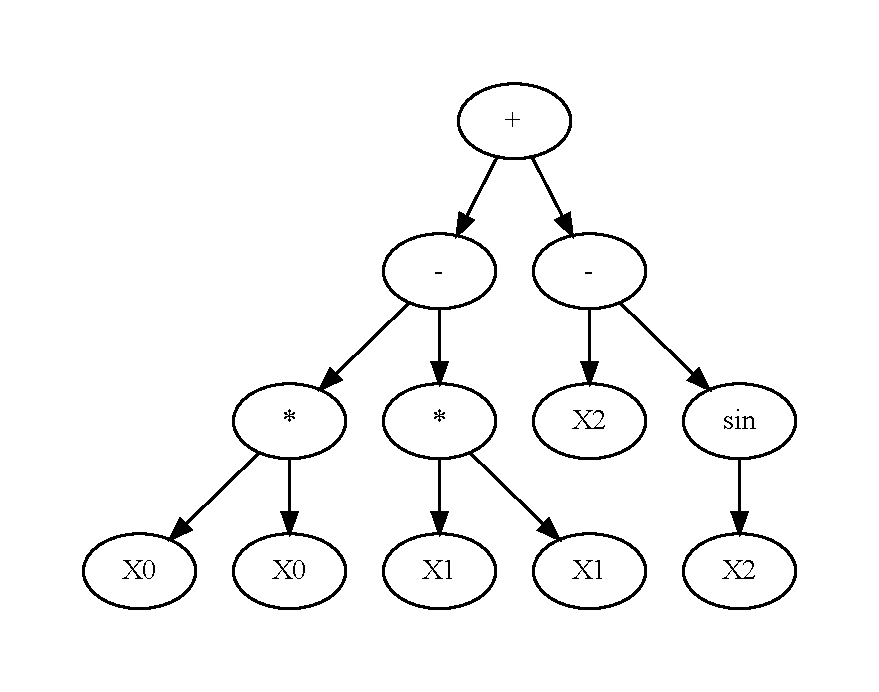
\includegraphics[scale=0.8]{images/graphviz/point_mut_before.dot.pdf}
    \caption{The original expression tree before performing a point mutation}
    \label{fig:point_muta}
  \end{subfigure}%
  \\
  \begin{subfigure}{\textwidth}
    \centering
    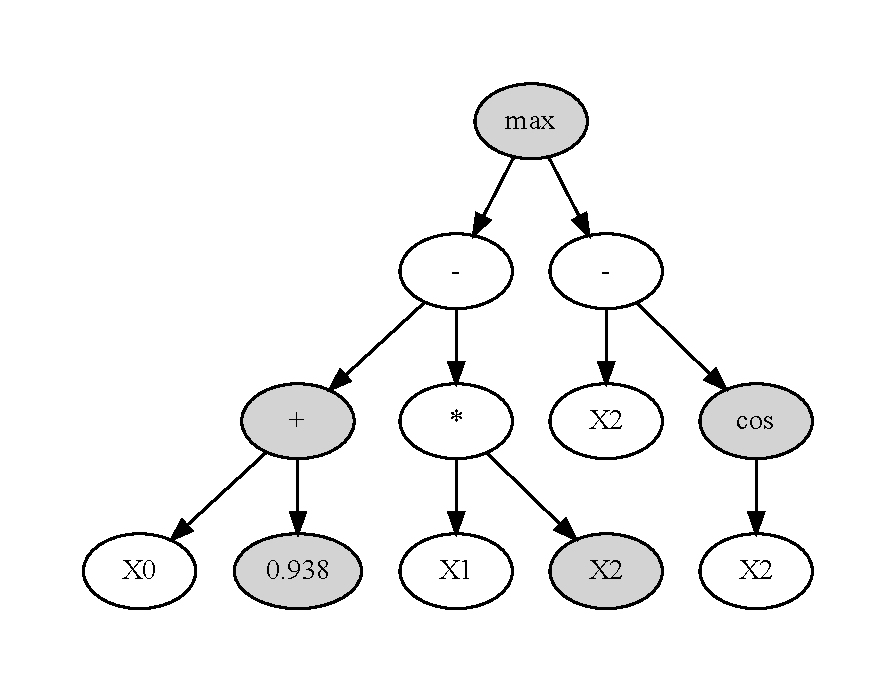
\includegraphics[scale=0.8]{images/graphviz/point_mut_after.dot.pdf}
    \caption{The same expression tree after a point mutation. The shaded nodes represent the changed terminals and functions in the final program.}
    \label{fig:point_mutb}
  \end{subfigure}
  \caption{Visualizing point mutations. Note that here, the program is the expression tree itself. }
  
  \label{fig:point}
\end{figure}

\subsubsection{Hoist Mutations}
\label{subsec:hoist}
In hoist mutations, we take the winner of a tournament and selects a random subtree from it. Another random subtree is selected from this subtree as a replacement for the subtree from the program. 

This mutation serves to reduce bloating of programs with increase in number of generations. \Cref{fig:hoist} visualizes the effect of hoist mutations on a given expression tree.

\begin{figure}[htp]
  \centering
  \begin{subfigure}{\textwidth}
    \centering
    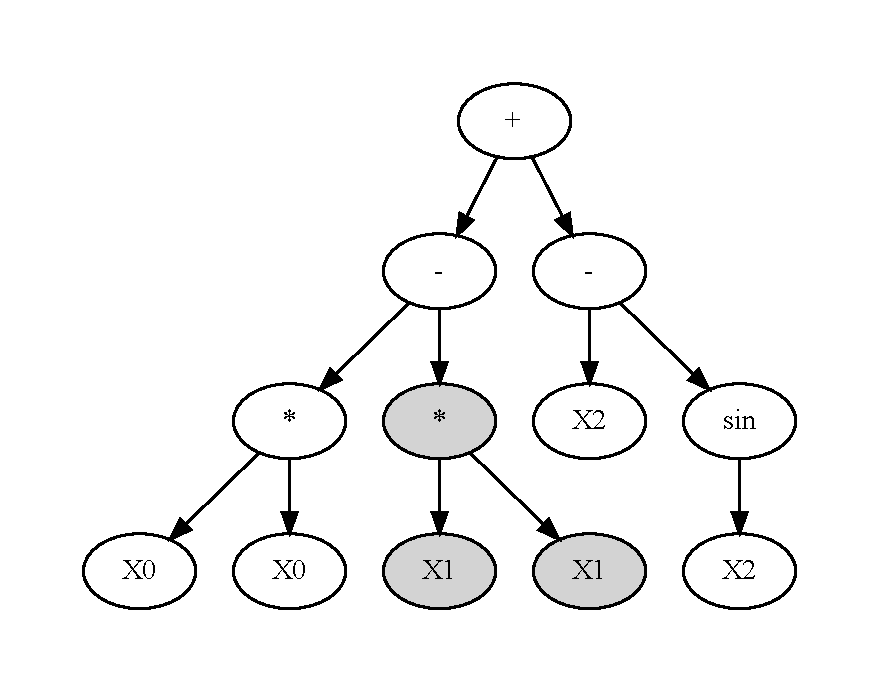
\includegraphics[scale=0.8]{images/graphviz/hoist_mut_before.dot.pdf}
    \caption{The original expression tree before performing a hoist mutation. The dark grey nodes denote the selected subtree, and the grey nodes denote the hoist subtree.}
    \label{fig:hoist_muta}
  \end{subfigure}%
  \\
  \begin{subfigure}{\textwidth}
    \centering
    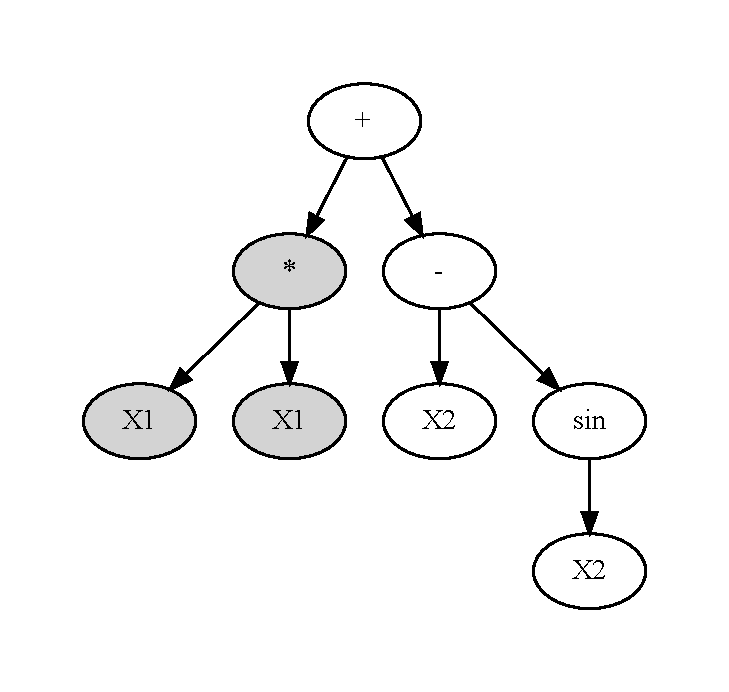
\includegraphics[scale=0.8]{images/graphviz/hoist_mut_after.dot.pdf}
    \caption{The same expression tree after hoisting the sub-subtree onto it's parent's position.}
    \label{fig:hoist_mutb}
  \end{subfigure}
  \caption{Visualizing hoist mutations for an expression tree. }
  
  \label{fig:hoist}
\end{figure}

\subsubsection{Crossover Mutations}
\label{subsec:crossover}
Crossover is a method of mixing genetic information between $2$ programs from a given population. In crossover mutations, we first determine a parent and a donor program using $2$ seperate tournaments. We then select a random subtree of the parent program. The child program for the next generation is generated by replacing this subtree with a random subtree from the donor program. 

Crossover is considered as the principle method for evolution in our implementation, which is again inspired by \citep{gplearn}. We show a sample visualization of the crossover operation in \cref{fig:crossover}.

\begin{figure}[htp]
  \centering
  \begin{subfigure}{\textwidth}
    \raggedleft
    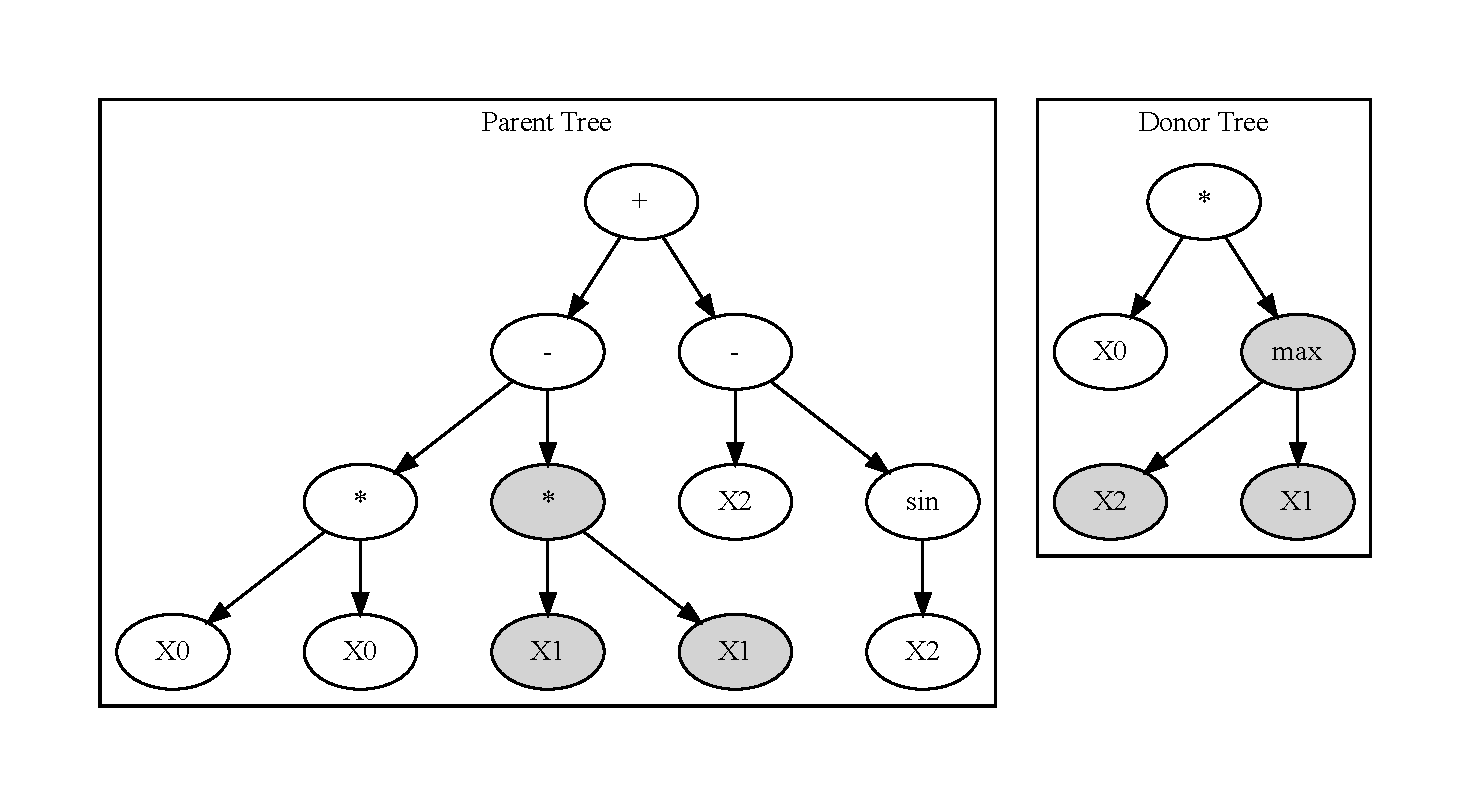
\includegraphics[scale=0.75]{images/graphviz/crossover_before.dot.pdf}
    \caption{The parent and donor expression trees, both selected through tournaments are shown here.}
    \label{fig:crossover_muta}
  \end{subfigure}%
  \\
  \begin{subfigure}{\textwidth}
    \centering
    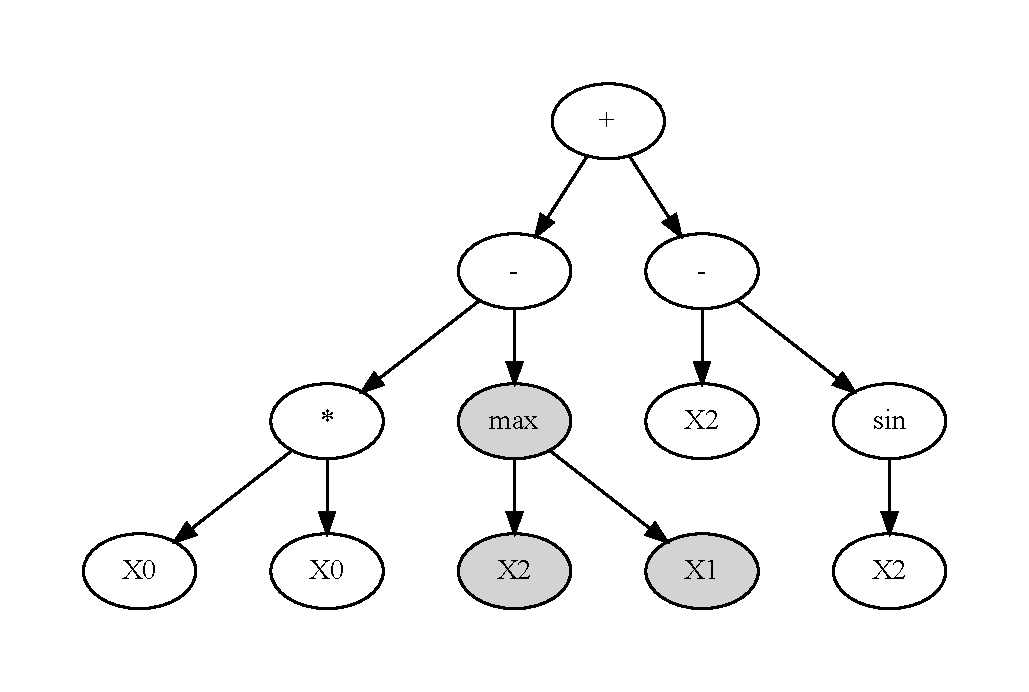
\includegraphics[scale=0.75]{images/graphviz/crossover_after.dot.pdf}
    \caption{The child expression tree after replacing a subtree of the parent with that of the donor.}
    \label{fig:crossover_mutb}
  \end{subfigure}
  \caption{Visualizing crossover mutations for a given parent and donor program.}
  
  \label{fig:crossover}
\end{figure}

\subsubsection{Subtree Mutations}
\label{subsec:subtree}
In subtree mutations, we perform a crossover between the winning parent tree and a randomly generated program. It serves as a method to increase new terminals and extinct functions in the next generation of programs, and is more agressive compared to a crossover mutation.\citep{gplearn} 

\Cref{fig:subtree} visualizes a sample subtree mutation in practice. We note that it is almost the same as the crossover visualization in \Cref*{fig:crossover}, with  the exception being that the donor tree in \cref*{fig:crossover_muta} is now a randomly generated tree in \cref*{fig:subtree_muta}. 

\begin{figure}[htp]
  \centering
  \begin{subfigure}{\textwidth}
    \raggedleft
    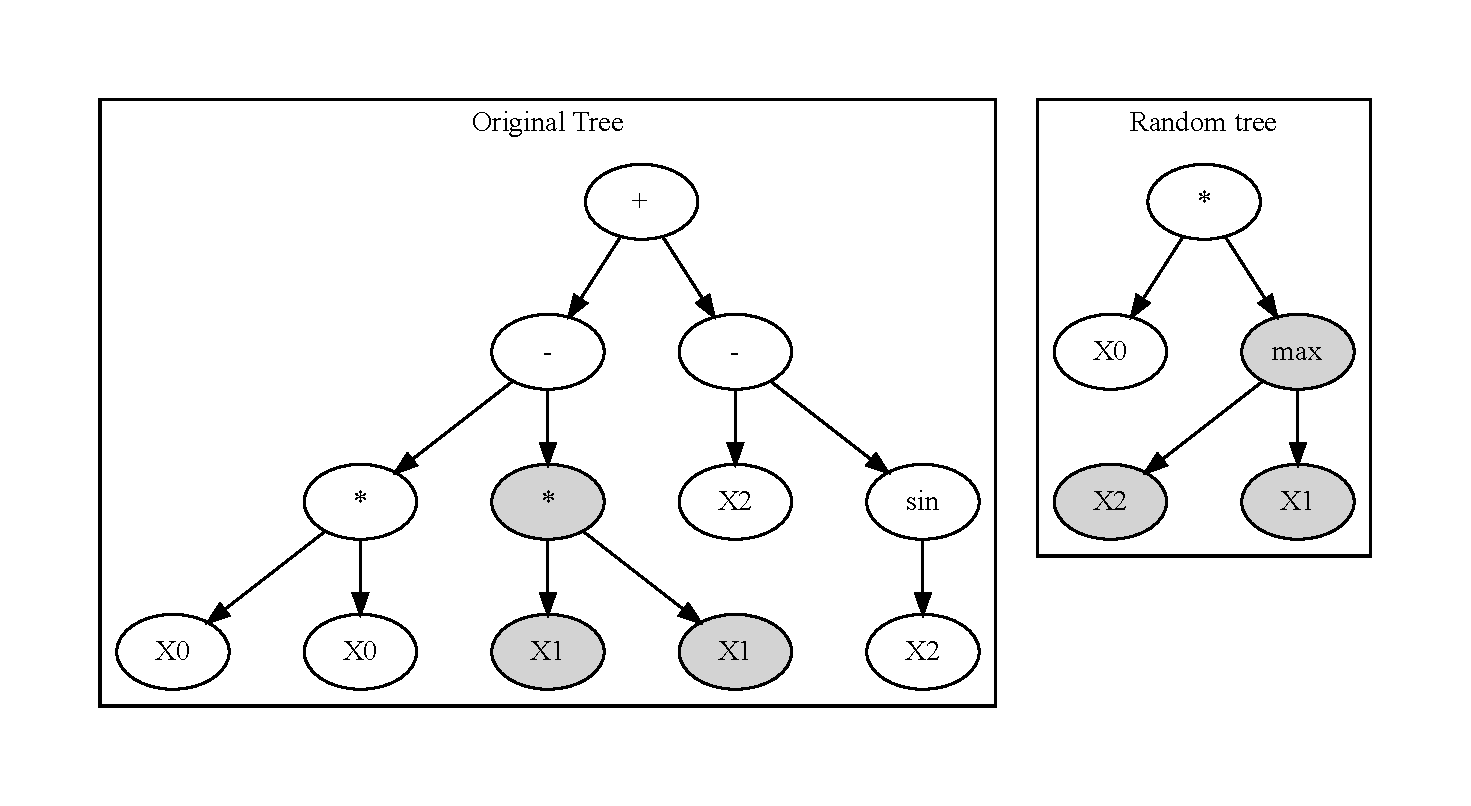
\includegraphics[scale=0.75]{images/graphviz/subtree_before.dot.pdf}
    \caption{The parent expression tree and a randomly generated tree is shown here.}
    \label{fig:subtree_muta}
  \end{subfigure}%
  \\
  \begin{subfigure}{\textwidth}
    \centering
    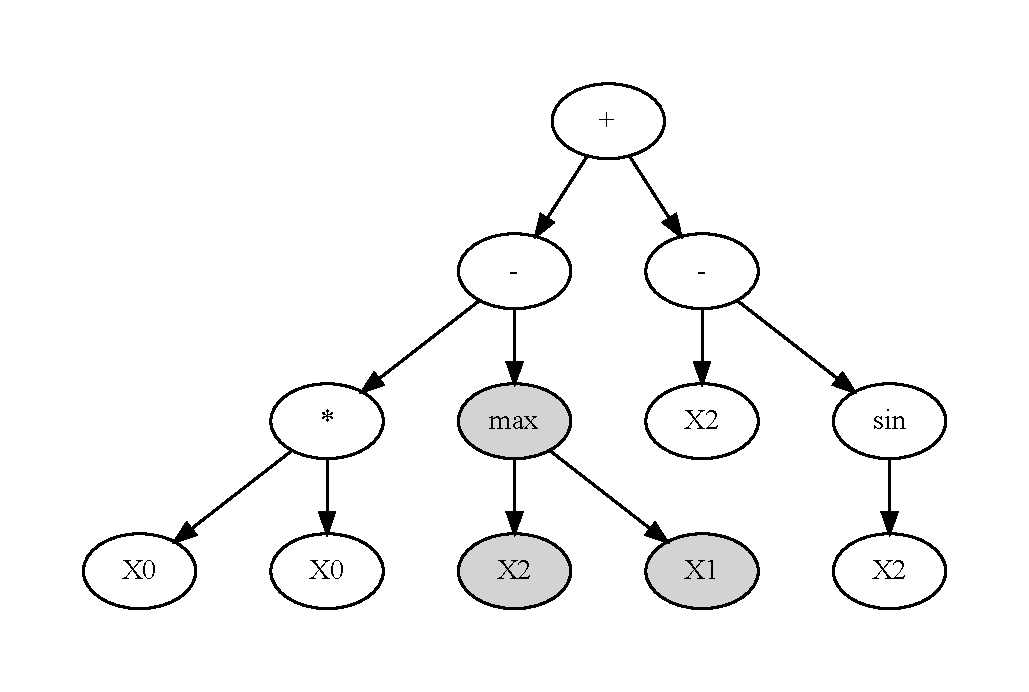
\includegraphics[scale=0.75]{images/graphviz/subtree_after.dot.pdf}
    \caption{The child expression tree after replacing a subtree of the parent with that of the random tree.}
    \label{fig:subtree_mutb}
  \end{subfigure}
  \caption{Visualizing subtree mutations for a given parent program.}
  
  \label{fig:subtree}
\end{figure}
  
\subsection{Evaluation}
\label{subsec:evaluation}
Once the population for the next generation is decided after selection and mutation, the fitness of all programs in the new generation is recomputed. This step is the major bottleneck when scaling the generational GP algorithm to bigger datasets and bigger populations, as the evaluation is independent for every program and every row of the input dataset. 

We perform the evaluation and computation of fitness in our implementation using a CUDA kernel and linear algebra primitives specified in the RAFT library(\citep{raschka2020machine}).

\section{Existing Libraries and Their Coverage}
\label{sec:otherlibs}
The table below(mostly reproduced from \cite{baeta2021speed}) lists some of the common libraries  used for genetic programming.  

\begin{table}[htbp]
  \caption{Existing GP frameworks along with language and device support}
  \begin{center}
      \begin{tabular}[c]{|c|c|c|}
          \hline
          \textbf{Framework} &   \textbf{Language} & \textbf{Compute Type} \\
          \hline
          KarooGP & python & CPU/GPU \\
          TensorGP & python & CPU/GPU \\
          DEAP & python & CPU \\
          gplearn  & python & CPU \\
          ECJ & Java & CPU \\
          \hline
      \end{tabular}
      \label{tab:otherlibs}
  \end{center}
\end{table}

Among the libraries listed in \cref{tab:otherlibs}, both TensorGP(\citep{baeta2021tensorgp}) and KarooGP(\citep{staats2017tensorflow}) use the TensorFlow python framework to perform fitness evaluation the GPU. However, while KarooGP uses TensorFlow's \textit{graph} execution model, where every program is compiled into a DAG wheras TensorGP uses TensorFlow's \textit{eager} execution model\citep{agrawal2019tensorflow}, where expressions are evaluated immediately without the overhead of graph construction. The GPU parallelization here is through the use of TensorFlow-based vectorization, and not the explicit use of CUDA. 

DEAP \citep{DEAP_JMLR2012} is another commonly used Evolutionary Computing framework in Python implements a parallelized version of the GP framework. However, it offers only CPU based parallelization. 

GPlearn\citep{gplearn} is another Python framework which provides a method to build GP models for symbolic regression, classification and transformation using an API which is compatible with scikit-learn\citep{scikit-learn}. It also provides support for running the evolutionary process in parallel. The base code that is parallelized on GPUs in this thesis is largely inspired by GPlearn. 

The ECJ Evolutionary Computing Toolkit\citep{Luke1998ECJSoftware} is a Java library for many popular EC algorithms, with a emphasis towards genetic programming. Almost all aspects of \cref{gpalgo} are governed by a hierarchy of user-provided parameter files and classes, and the framework itself is designed for large, heavyweight experimental needs. Using ECJ parameter files, it is also possible to define custom GP pipelines with user-defined evolution strategies.

In the next chapter, we will talk about our work on parallelizing the GP algorithm to perform symbolic regression.